  
%情報処理学会全国大会原稿テンプレート ver. 1.2

\documentclass[uplatex,twocolumn]{jsarticle}
\usepackage[top=30mm,bottom=25mm,left=20mm,right=20mm]{geometry}
\usepackage[T1]{fontenc}
\usepackage{txfonts}
\usepackage[expert,deluxe]{otf}
\usepackage[dvipdfmx,hiresbb]{graphicx}
\usepackage[dvipdfm]{hyperref}
\usepackage{pxjahyper}
\usepackage{multicol}
\usepackage{here}
\setlength{\columnsep}{7mm}

\title{\vspace{-10mm}動画投稿サービスにおける有料コメントシステムの利用に関する調査\footnotemark[0]}
\author{\large{島田 光馬\footnotemark[2]\qquad 矢吹 太朗}\\千葉工業大学 社会システム科学研究科 マネジメント工学専攻\footnotemark[3]}
\date{}
\pagestyle{empty}
\begin{document}
\twocolumn[\maketitle]

\begingroup
\def\thefootnote{\fnsymbol{footnote}}
\footnotetext[0]{Survey on the use of paid commenting systems in video posting services.}
\footnotetext[2]{Mitsuma SHIMADA (\verb|s1542052fb@s.chibakoudai.jp|)}
\footnotetext[3]{Graduate School of Social Systems Science, Department of Management Engineering. Chiba Institute of Technology.}
\endgroup

\section{序論}

動画閲覧サイトでは,ビデオ内に広告を表示するIn-Video広告と呼ばれる提示形式が使用されている.In-Video広告は動画を視聴する妨げとなるため,不快に感じるユーザがいる\cite{01}..
そのため,動画サイトの一つであるYouTubeでは広告はスキップされることがある.広告がスキップされると,配信者が広告費収入を得られなくなる.配信者にとっては,配信者が広告収入を得るための審査が厳しかったり,広告が掲載されなくなる基準が不透明であるという問題もある.そこで,広告ではなく,視聴者から直接対価を受け取れるしくみが広まってきている.YouTubeでは,そのしくみはスーパーチャット(以下,スパチャという)である.


YouTubeの魅力は,主にコミュニケーションツールとしてテキストを使用される\cite{02}.
YouTubeに動画を流した場合,視聴者がコメントをしてクリエイターの質を上げている.さらに,ライブ配信をするとリアルタイムで視聴者とコミュニケーションが取れることも魅力である.スパチャをする視聴者のほとんどは,クリエイターのファンが多いため,日本でのVtuberに投資する人も存在する.

2017年の当時では,米国で配信者にヘイトスピーチを送るために投げ銭をする人が多いが,日本ではアイドルのような形で投げ銭を行う人が増えた.
YouTubeのスパチャ累計額TOP20では,日本のVtuberが16人ランクインしている\cite{03}.
世界でも,日本のVtuberが検索され視聴されていることから,スパチャとコメントの関係性があるのではないかと考えた.

Vtuberとは,VirtualYouTuberの略で,コンピュータグラフィックスで日本発祥のキャラクター(アバター)を用いて動画投稿・配信を行う人である.

ライブ配信サービスでよく使われている投げ銭について調査した.


\section{目的}

ライブ配信サービスにおける投げ銭システムを収集するためのツールを開発し,それを用いて配信者別にコメントに対して投げ銭が多いか調査する.

\section{手法}

本研究は以下の3段階で行う.

\begin{enumerate}
 \item YouTubeライブ配信のアーカイブからコメントとスパチャを取り出すためのツールを開発する.
 \item ライブ配信のチャットログからスパチャとコメントを集計する.
 \item コメントと時間,スパチャをヒストグラムで表す.
\end{enumerate}

初めに,YouTubeにライブ配信しているクリエイターのアーカイブからチャットログを収集する.YouTube APIでは,チャットログの制限で1日500件程度しか取得することが出来ないという制限があるため,本研究では使えない\cite{04}.そこで,ブラウザの操作を自動化するためのフレームワークとして,「selnium」を使用し,インターネットブラウザ上のYouTubeでクリエイターが残したページから,チャットログのデータを取得する.

次に,取得したデータはjson形式として保存されているため,「コメント件数,スパチャ件数,コメント投稿時間,スパチャ投稿時」を取り出すツールを作成する.

最後に,「コメント件数,スパチャ件数,コメント投稿時間,スパチャ投稿時間」から,スパチャとコメントに対する投稿した時間を使って,分析を行う.

本調査では,YouTube上のURLを取りだすことで「コメント件数,スパチャ件数,コメント投稿時間,スパチャ投稿時間」を抜き取る.

\section{結果}

ツールを作成した際,数か月おきにYouTubeでシステムアップデートが行われており,常に対応できる最新のツールにする必要があった.そのため,selniumを使用し,随時取れるツールを開発した.
データを取得するクリエイターのアーカイブを見つけ,チャットログが表示されている配信からデータを取得する.
取得したデータでは,コメントと時間,スパチャを取得している.
図1では,取得したスパチャの累計金額を時間でグラフ化し,図2のように金額をヒストグラムで阿波らしている.表3は,スパチャに対する統計量を表している.

\begin{figure}[H]
%\includegraphics[width=図の幅,clip]{ファイル名}\label{参照用ラベル}
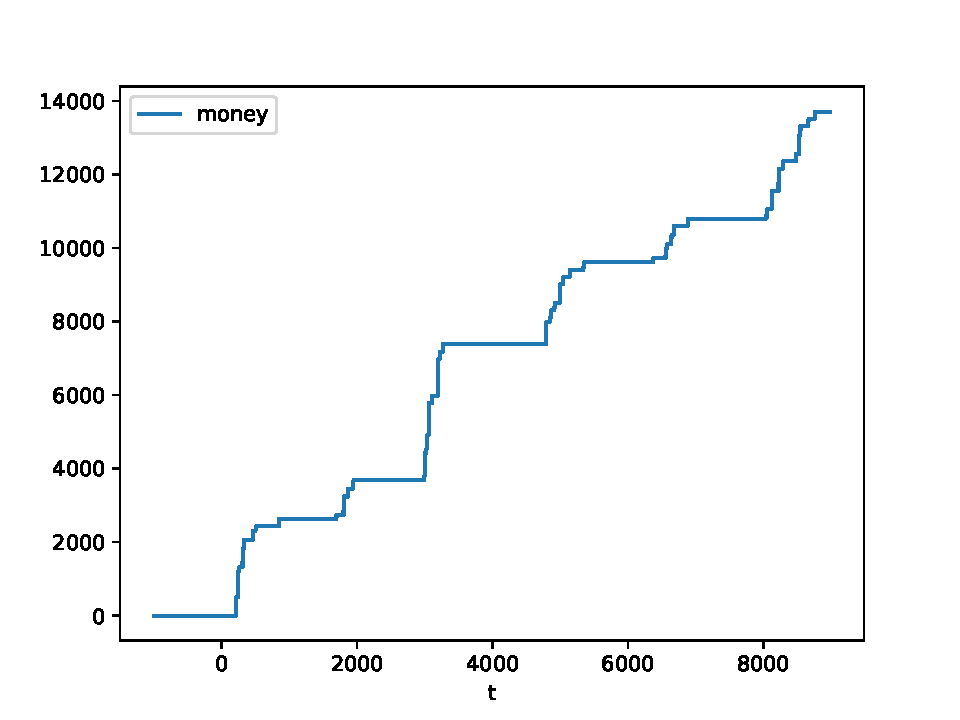
\includegraphics[width=8cm,clip]{livechatlog.pdf}
\caption{放送時間に対する累計金額}\label{time}
\end{figure}

\begin{figure}[H]
%\includegraphics[width=図の幅,clip]{ファイル名}\label{参照用ラベル}
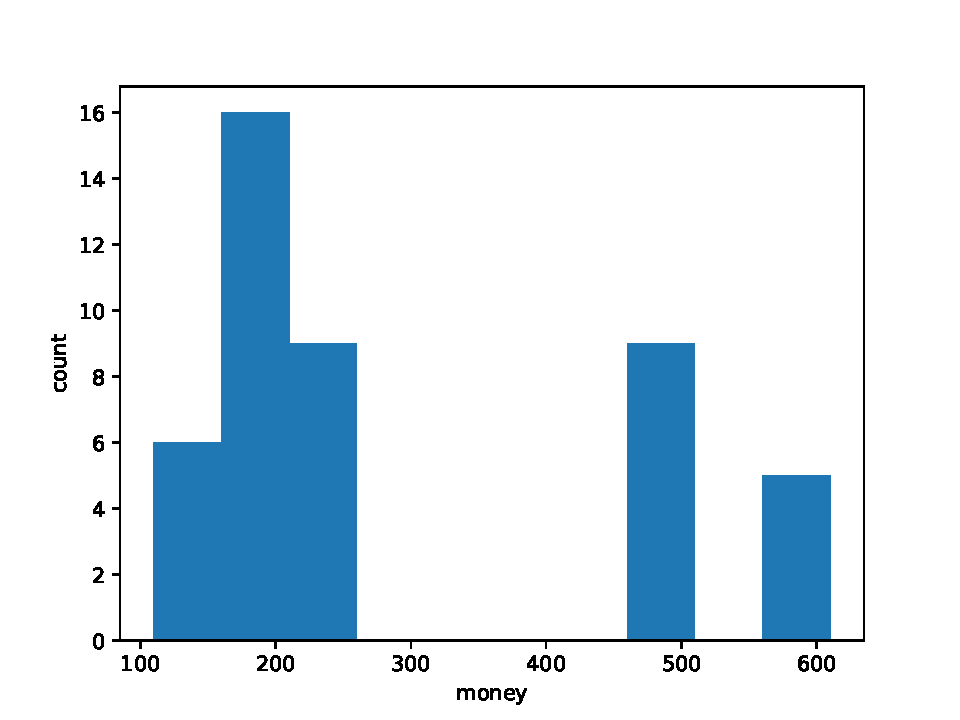
\includegraphics[width=8cm,clip]{livechatlog_hist.pdf}
\caption{スパチャ件数に対する金額}\label{hist}
\end{figure}

\begin{table}[hbtp]
\caption{放送時間に対する累計金の統計量}
\label{table:data_type}
\centering
\begin{tabular}{lcr}
\hline
count & 45.000000 \\
mean & 304.666667 \\
std & 166.523272 \\
min & 110.000000 \\
25% & 200.000000 \\
50% & 250.000000 \\
75% & 500.000000 \\
max & 610.000000 \\
Name: 9 & dtype: float64 \\
\hline
\end{tabular}
\end{table}




\section{考察}
調査した結果,スパチャには,円やドル,ユーロなど様々なお金が存在する.
データでは,Vtuberを対象としているため比較的に円がほとんどだったが,中にはドルやユーロも見かけた.
各配信ごとに統計は変わっており,平均が2,000を超えることもある.

スパチャの累計が跳ね上がっている個所は,コメントが秒単位で何千件も送られている.中には,英語で感謝の言葉を添えている視聴者も存在した.このことから,配信をすることは,国際的なコミュニケーションが成立している.

\section{結論}
まず,投げ銭のログをとるシステムを開発した.

YouTube apiでは制限がかかり使えず,投げ銭システムを収集するツールの開発を行った.
開発したシステムを使って投げ銭のログを取得し,基本的な統計量を調査した.大量の動画への投げ銭を解析し,投げ銭を受ける配信者の特徴や,投げ銭を投げる視聴者の特徴を調べることが今後の課題である.


\bibliographystyle{junsrt}
\bibliography{biblio}%「biblio.bib」というファイルが必要.


\end{document}